\begin{center}
\large\noindent\fbox{
	\parbox{\textwidth}{
	Utilizzare la function dell'Esercizio 4.1 per approssimare la funzione di Runge sull'intervallo \([-6,6]\), su una partizione uniforme di \(n+1\) ascisse per \(n = 2,4,6, \ldots,40\). Stimare le corrispondenti costanti di Lebesgue.
	}
}\end{center}

\noindent Il seguente codice Matlab contiene la soluzione al problema dato:

\lstinputlisting[language=Matlab]{Codici/Cap4/Esercizio9_Cap4.m}

\pagebreak
\noindent Di seguito i grafici mostrano i polinomi interpolanti di Lagrange al variare del grado  $N$ con \(N = 2,4,6, \ldots,40\).

\begin{figure}[H]
	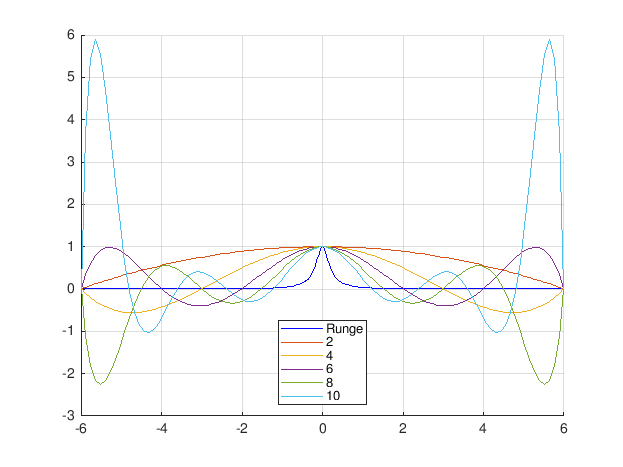
\includegraphics[height=0.6\textwidth,width=\textwidth]{Codici/Cap4/es9(n10)}
\end{figure}

\begin{figure}[H]
	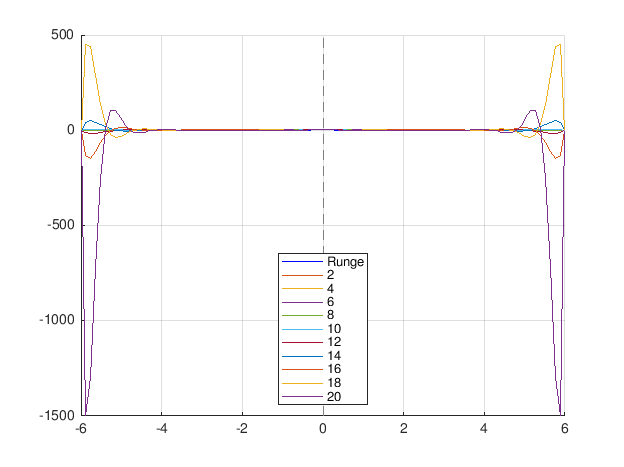
\includegraphics[width=\textwidth]{Codici/Cap4/es9(n20)}
\end{figure}

\begin{figure}[H]
	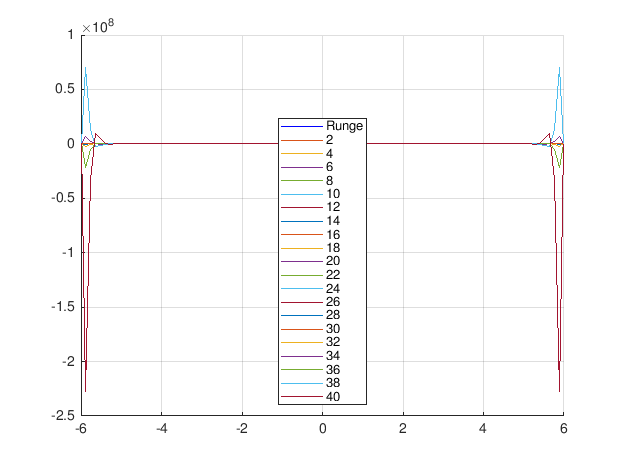
\includegraphics[height=0.6\textwidth,width=\textwidth]{Codici/Cap4/es9(n40)}
\end{figure}

Nella tabella è riportato come varia la \textit{costante di Lebesgue}, al variare del grado \textit{n} del polinomio interpolante. Come si può vedere, all'aumentare di \textit{n} l'errore aumenta a causa della scelta delle ascisse equispaziate.

\begin{center}
	\begin{tabular}{|c|c|}
		\hline
		$n$ & $lebesgue$ \\
		\hline
		$2$  & $0.9342$ \\ 
		$4$  & $0.8566$ \\ 
		$6$  & $0.9846$ \\ 
		$8$  & $2.2590$ \\ 
		$10$ & $5.8960$ \\ 
		$12$ & $16.3788$ \\ 
		$14$ & $49.2750$ \\ 
		$16$ & $147.6550$ \\ 
		$18$ & $450.3933$ \\ 
		$20$ & $1.5025e+03$ \\ 
		$22$ & $5.0066e+03$ \\ 
		$24$ & $1.6654e+04$ \\ 
		$26$ & $5.5282e+04$ \\ 
		$28$ & $1.8307e+05$ \\ 
		$30$ & $6.0468e+05$ \\ 
		$32$ & $1.9918e+06$ \\ 
		$34$ & $6.5422e+06$ \\ 
		$36$ & $2.1426e+07$ \\ 
		$38$ & $6.9960e+07$ \\ 
		$40$ & $2.2774e+08$ \\ 
		\hline
	\end{tabular}
\end{center}